
%! program = pdflatex

\documentclass[12pt]{article}
\usepackage{amsmath}
\usepackage{natbib}
\usepackage{graphicx}
\usepackage{amssymb}
\usepackage{epstopdf}
\usepackage{float} % to keep the figures in place

\usepackage{color}
\newcommand{\cred}{ \color{red}}
\newcommand{\cgreen}{\color{green}}
\newcommand{\cblue}{\color{blue}}
\newcommand{\cmag}{\color{magenta}}
\newcommand{\bn}{\begin{enumerate}}
\newcommand{\en}{\end{enumerate}}
\newcommand{\bi}{\begin{itemize}}
\newcommand{\ei}{\end{itemize}}
\newcommand{\be}{\begin{eqnarray}}
\newcommand{\ee}{\end{eqnarray}}
\newcommand{\by}{\begin{eqnarray*}}
\newcommand{\ey}{\end{eqnarray*}}
\renewcommand{\labelenumi}{(\alph{enumi}) }
%
\usepackage[margin=2.2cm, includehead]{geometry}% see geometry.pdf on how to lay out the page. There's lots.
\geometry{letterpaper} % or letter or a5paper or ... etc
% \geometry{landscape} % rotated page geometry
%\bibpunct{(}{)}{;}{a}{,}{,}
%\setlength{\textwidth}{16cm}
%\setlength{\textheight}{21cm}
\def\nonumber{\global\@eqnswfalse}
\newcounter{parnum}
\newcommand{\N}{%
  \noindent\refstepcounter{parnum}%
   \makebox[\parindent][l]{\textbf{[\arabic{parnum}]}}\quad  }
% Use a generous paragraph indent so numbers can be fit inside the
% indentation space.
\setlength{\parindent}{1.5em}

% See the ``Article customise'' template for come common customisations

\date{}
%\date{} % delete this line to display the current date

%%% BEGIN DOCUMENT
\usepackage{Sweave}
\begin{document}
\Sconcordance{concordance:HW1.tex:HW1.Rnw:%
1 47 1 1 0 64 1 1 8 1 2 4 1 1 6 1 2 4 1 1 6 1 2 5 1 1 7 1 2 63 1 1 8 1 %
2 4 1 1 4 1 2 45 1 1 8 1 2 5 1 1 6 1 2 35 1 1 21 1 2 4 1 1 6 1 2 4 1 1 %
6 1 2 10 1 1 5 1 2 6 1 1 6 3 0 1 3 3 0 1 2 4 1 1 6 3 0 1 3 3 0 1 2 3 1 %
1 7 4 0 1 2 9 1 1 4 1 2 6 1 1 4 3 0 1 3 3 0 1 2 1 1 1 6 3 0 1 1 3 0 1 2 %
2 1 1 4 3 0 1 3 3 0 1 2 3 1 1 2 4 0 1 2 1 9 4 0 1 2 5 1 1 6 8 0 1 2 1 6 %
5 0 1 2 1 6 7 0 1 2 1 6 7 0 1 2 1 6 4 0 1 2 1 6 7 0 1 2 1 1}

%\large
%\maketitle
\newtheorem{thm}{Theorem}[section]
\newtheorem{cor}[thm]{Corollary}
\newtheorem{lem}[thm]{Lemma}
\newtheorem{prop}[thm]{Proposition}
\newtheorem{defn}[thm]{Definition}
\newtheorem{exam}[thm]{Example}
\newtheorem{qstn}[thm]{Question}

%%%
\newpage
\begin{center}
{\bf Homework 1 - STAT 511}\\
Amal Agarwal
\end{center}
%==========================
\section*{Answer 1}
\bn
\item Y$\sim$ Binom$(n,p), y\in \left\{0,1,2,...\right\}$\\
Probability mass function (pmf) of Y is\\
$P(Y=y)={n \choose y}p^y(1-p)^{(n-y)}, y\in \left\{0,1,2,...\right\}$\\
Now the mean can be evaluated as 
\begin{equation*}
\begin{aligned}
E[Y] &= \sum\limits_{y=0}^\infty yP(Y=y)\\
&= \sum\limits_{y=0}^\infty y{n \choose y}p^y(1-p)^{(n-y)}\\
&= \sum\limits_{y=0}^\infty y\frac{n!}{y!(n-y)!}p^y(1-p)^{(n-y)}\\
&= \sum\limits_{y=0}^\infty \frac{n(n-1)!}{(y-1)!(n-y)!}pp^{(y-1)}(1-p)^{(n-y)}\\
&= np\sum\limits_{y=1}^\infty \frac{(n-1)!}{(y-1)!(n-y)!}p^{(y-1)}(1-p)^{(n-y)}\\
&= np\sum\limits_{y=1}^\infty {n-1 \choose y-1}p^{(y-1)}(1-p)^{(n-y)}\\
&= np \left(\because \sum\limits_{y=1}^\infty {n-1 \choose y-1}p^{(y-1)}(1-p)^{(n-y)}=\sum\limits_{x=0}^\infty {n-1 \choose x}p^{(x)}(1-p)^{(n-1-x)}=1\right)
\end{aligned}
\end{equation*}
\setlength{\belowdisplayskip}{0pt}
Similarily
\begin{equation*}
\begin{aligned}
E[Y^2] &=\sum\limits_{y=0}^\infty y^2P(Y=y)\\
&= \sum\limits_{y=0}^\infty y^2{n \choose y}p^y(1-p)^{(n-y)}\\
&= \sum\limits_{y=0}^\infty y^2\frac{n!}{y!(n-y)!}p^y(1-p)^{(n-y)}\\
&= \sum\limits_{y=0}^\infty (y-1+1)\frac{n(n-1)!}{(y-1)!(n-y)!}p^y(1-p)^{(n-y)}\\
&= \sum\limits_{y=0}^\infty (y-1)\frac{n(n-1)(n-2)!}{(y-1)!(n-y)!}p^y(1-p)^{(n-y)}+\sum\limits_{y=0}^\infty \frac{n(n-1)!}{(y-1)!(n-y)!}p^y(1-p)^{(n-y)}\\
&= \sum\limits_{y=0}^\infty \frac{n(n-1)(n-2)!}{(y-2)!(n-y)!}p^2p^{(y-2)}(1-p)^{(n-y)}+\sum\limits_{y=0}^\infty \frac{n(n-1)!}{(y-1)!(n-y)!}pp^{(y-1)}(1-p)^{(n-y)}\\
&= n(n-1)p^2\sum\limits_{y=2}^\infty \frac{(n-2)!}{(y-2)!(n-y)!}p^{(y-2)}(1-p)^{(n-y)}+np\sum\limits_{y=1}^\infty \frac{(n-1)!}{(y-1)!(n-y)!}p^{(y-1)}(1-p)^{(n-y)}\\
&= n(n-1)p^2+np\\
&= n^2p^2-np^2+np
\end{aligned}
\end{equation*}

Thus 
\begin{equation*}
\begin{aligned}
Var[Y]&=E[Y^2]-(E[Y])^2\\
&= (n^2p^2-np^2+np)-(np)^2\\
&= np-np^2\\
&= np(1-p)
\end{aligned}
\end{equation*}
\item If $E[Y]=np=3, Var[Y]=np(1-p)=3(1-p)=1 \Rightarrow p=\frac{2}{3}$ and $n=\frac{9}{2}$. But $n$ has to be a natural number and thus here the variance can't be made equal to $1$
\item Here the variance can't be made equal to 1. Suppose we make $n=5$ and $p=3/5$. With these parameters, the mean is again $3$ but the variance modifies to $6/5$. Taking these parameters, the plot and histogram of simulated random variables are:

\begin{figure}[H]
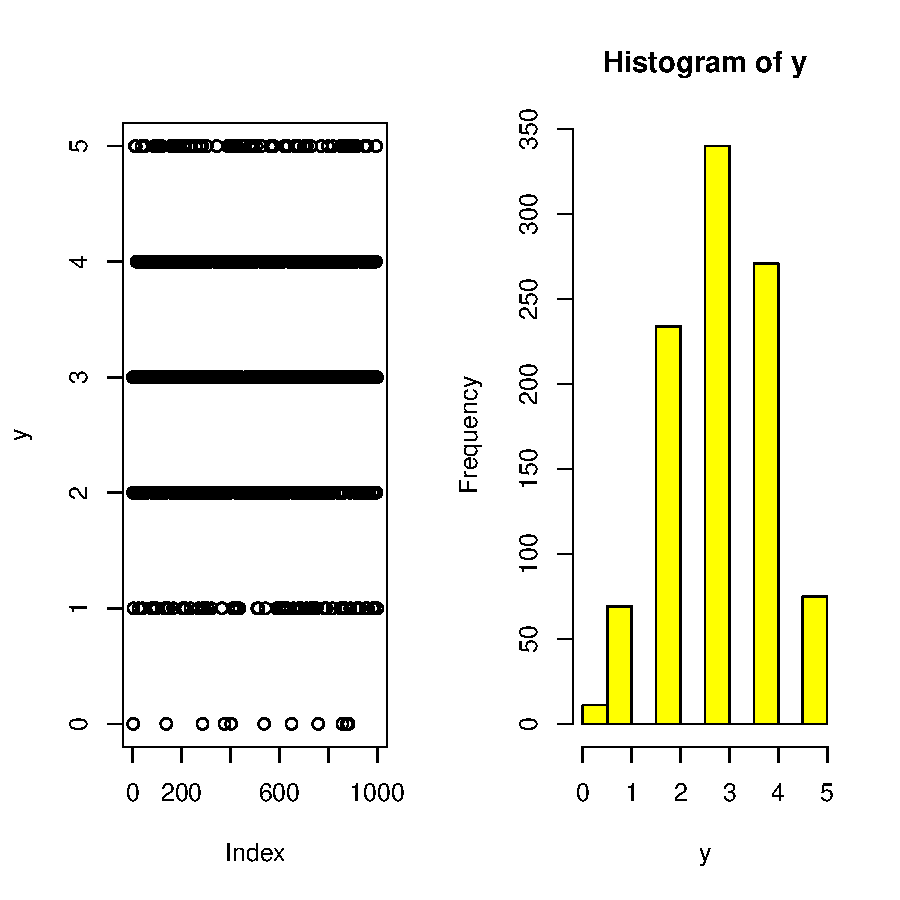
\includegraphics{HW1-001}
\end{figure}

\clearpage
\item The square root power transformation gives the following plots:
\begin{figure}[H]
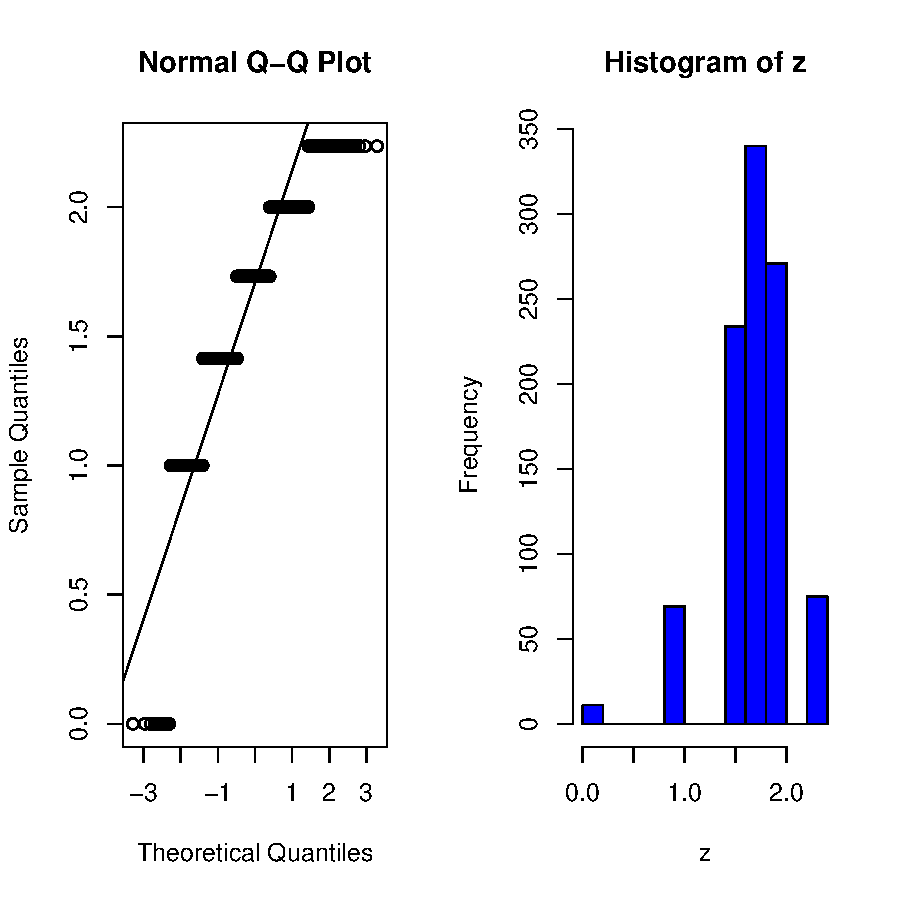
\includegraphics{HW1-002}
\end{figure}

\clearpage
The cube root power transformation gives the following plots:
\begin{figure}[H]
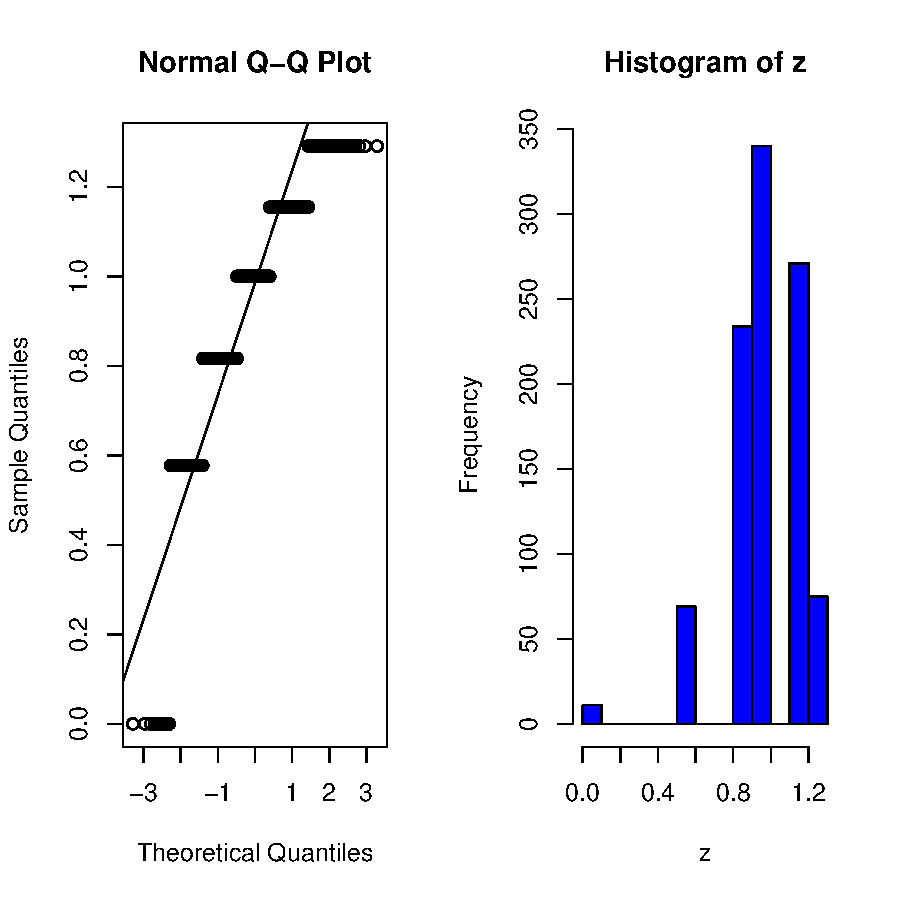
\includegraphics{HW1-003}
\end{figure}
\en

These qq plots show that even after the square root and cube root transformations, the data is far from being normally distributed. This is expected since binomial is a discrete distribution. However if we increase $n$ to $50$ and plot the graphs again, we get

\begin{figure}[H]
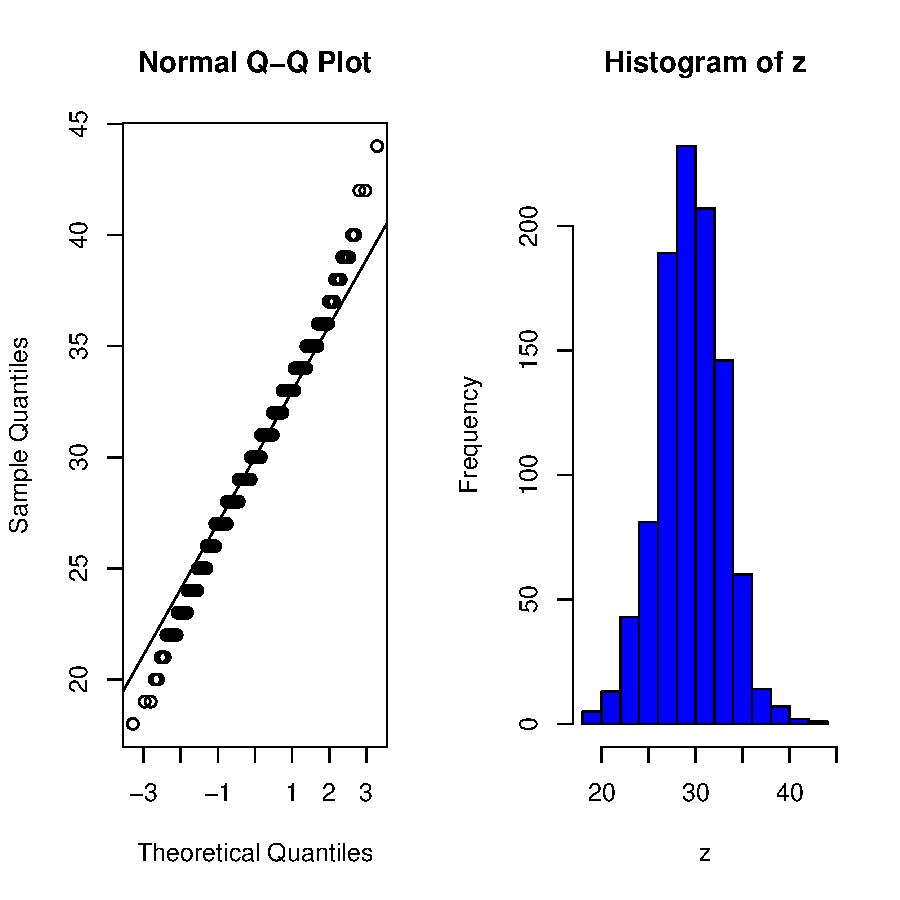
\includegraphics{HW1-004}
\end{figure}
 
This is significantly better which demonstrates the well known result that if $n\rightarrow \infty$, binomial distribution becomes close to normal.
%break

\section*{Answer 2}
\bn
\item Y$\sim$ Normal$(\mu, \sigma^2), y\in R$\\
Probability density function (pdf) of Y is\\
$f(y)=\frac{1}{\sqrt{2\pi\sigma^2}}e^{-\frac{(y-\mu)^2}{2\sigma^2}}, y\in R$\\
Now the mean can be evaluated as 
\begin{equation*}
\begin{aligned}
E[Y] &= \int_{-\infty}^{+\infty} \!yf(y)\ \mathrm{d}y \\
&= \int_{-\infty}^{+\infty} \!y\frac{1}{\sqrt{2\pi\sigma^2}}e^{-\frac{(y-\mu)^2}{2\sigma^2}}\ \mathrm{d}y \\
\end{aligned}
\end{equation*}
Assume $\frac{y-\mu}{\sqrt{2\sigma^2}}=x$ Thus we get
\begin{equation*}
\begin{aligned}
E[Y] &= \frac{1}{\sqrt{2\pi\sigma^2}}\int_{-\infty}^{+\infty} \!\sqrt{2\sigma^2}(\mu+\sqrt{2\sigma^2}x)e^{-x^2}\ \mathrm{d}x \\
&= \frac{1}{\sqrt{\pi}}\left[\int_{-\infty}^{+\infty} \!\mu e^{-x^2}\ \mathrm{d}x+\int_{-\infty}^{+\infty} \!\sqrt{2\sigma^2}x e^{-x^2}\ \mathrm{d}x\right] \\
\end{aligned}
\end{equation*}
The second integrand is an odd function and thus the integral from $-\infty$ to $+\infty$ goes to zero. Thus we have

\begin{equation*}
\begin{aligned}
E[Y] &= \frac{1}{\sqrt{\pi}}\left[\int_{-\infty}^{+\infty} \!\mu e^{-x^2}\ \mathrm{d}y \right] \\
&= \frac{1}{\sqrt{\pi}}\mu\sqrt{\pi}\\
&= \mu
\end{aligned}
\end{equation*}
Similarily
\begin{equation*}
\begin{aligned}
E[Y^2] &= \frac{1}{\sqrt{2\pi\sigma^2}}\int_{-\infty}^{+\infty}\!y^2e^{-\frac{(x-\mu)^2}{2\sigma^2}}\ \mathrm{d}y
\end{aligned}
\end{equation*}
Now substituting $y-\mu=t$
\begin{equation*}
\begin{aligned}
E[Y^2] &= \frac{1}{\sqrt{2\pi\sigma^2}}\left[\int_{-\infty}^{+\infty}\!t^2e^{-\frac{t^2}{2\sigma^2}}\ \mathrm{d}t+2\mu\int_{-\infty}^{+\infty}\!te^{-\frac{t^2}{2\sigma^2}}\ \mathrm{d}t+\mu^2\int_{-\infty}^{+\infty}\!e^{-\frac{t^2}{2\sigma^2}}\ \mathrm{d}t\right]
\end{aligned}
\end{equation*}
The second integral again goes to zero. Thus we obtain
\begin{equation*}
\begin{aligned}
E[Y^2] &= \frac{1}{\sqrt{2\pi\sigma^2}}\left[\frac{\sqrt{\pi}}{2}(2\sigma^2)^{3/2}+\mu^2\sqrt{2\pi\sigma^2}\right]
&= \sigma^2+\mu^2
\end{aligned}
\end{equation*}
Hence
\begin{equation*}
\begin{aligned}
Var[Y]&=E[Y^2]-(E[Y])^2\\
&= (\sigma^2+\mu^2)-(\mu)^2
&= \sigma^2
\end{aligned}
\end{equation*}
\item The set of parameters $(\mu, \sigma^2)$ that make $E[Y]=3$ and $Var[Y]=1$ are $(3,1)$.
\item If $E[Y]=\mu=3, Var[Y]=\sigma^2=1$, the plots of the simulated random variables and the histogram are given as:

\begin{figure}[H]
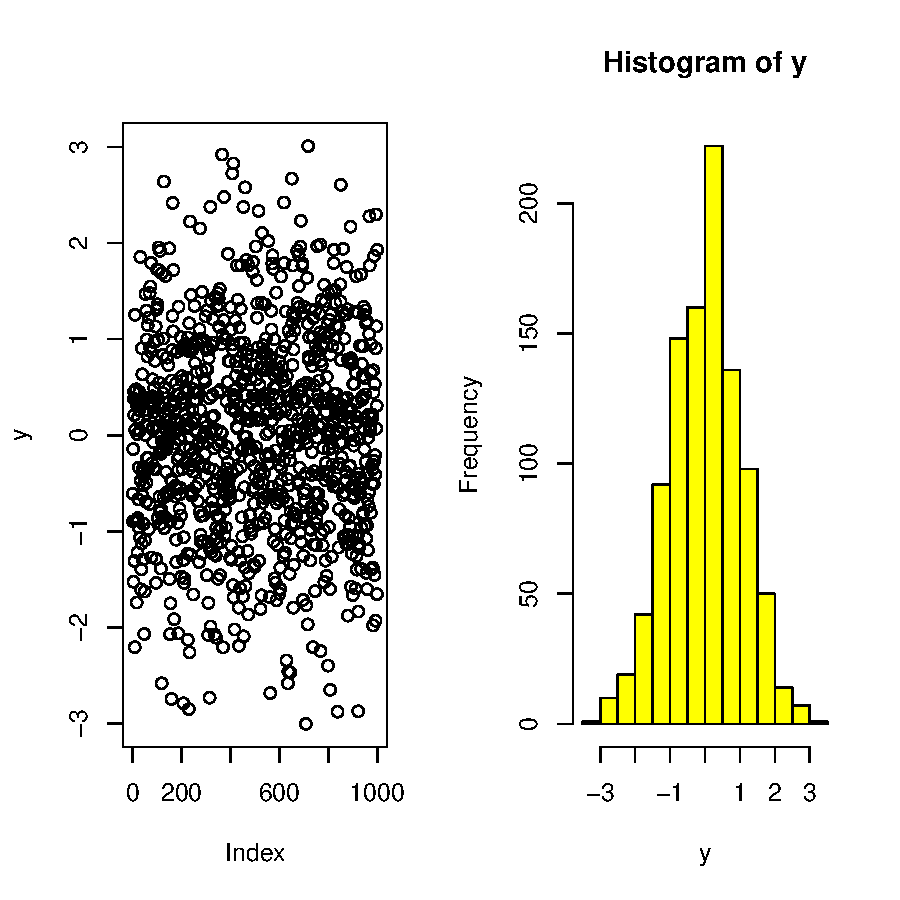
\includegraphics{HW1-005}
\end{figure}

\item Since this simulation is done for the normal distribution itself, no transformation is required to make it normal. The qq plot is given as 

\begin{figure}[H]
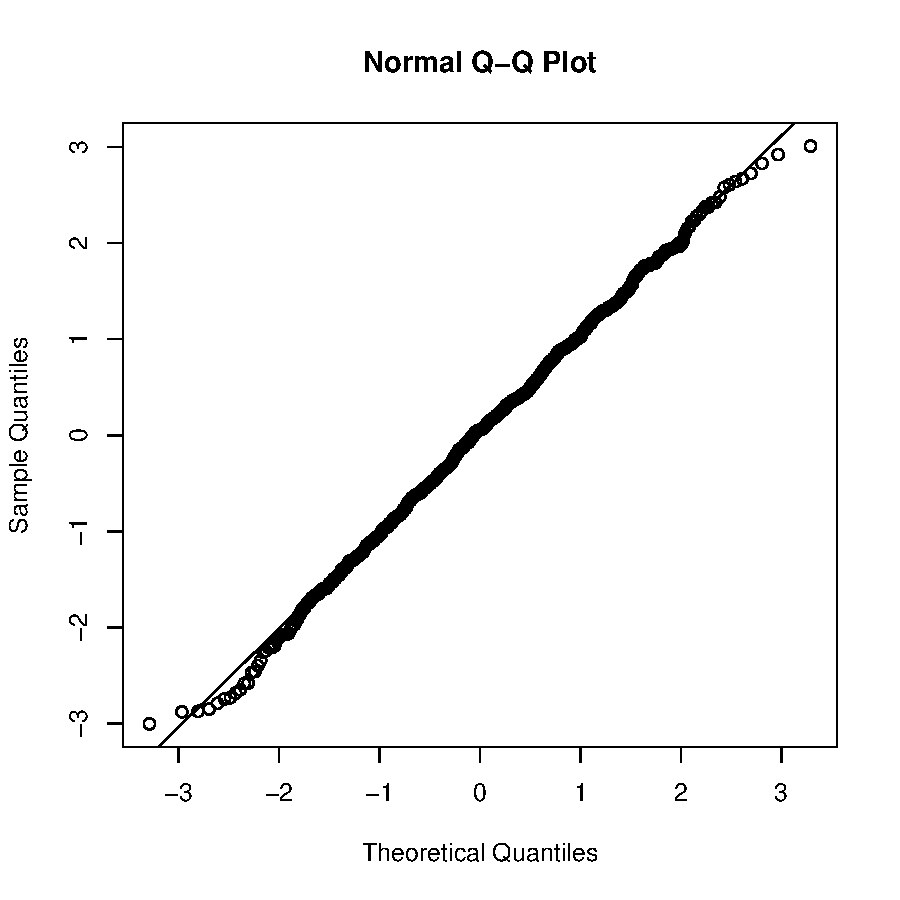
\includegraphics{HW1-006}
\end{figure}

\en

% break
\clearpage
\section*{Answer 3}
\bn
\item Y$\sim$ Poisson$(\lambda), y\in \left\{0,1,2,...\right\}$\\
Probability mass function (pmf) of Y is\\
$P(Y=k|\lambda)=\frac{\lambda^{k}}{k!}e^{-\lambda}, y\in \left\{0,1,2,...\right\}$\\
Now the mean can be evaluated as 
\begin{equation*}
\begin{aligned}
E[Y] &= \sum\limits_{k=0}^\infty kP(Y=k)\\
&= \sum\limits_{k=0}^\infty k\frac{\lambda^{k}}{k!}e^{-\lambda}\\
&= \sum\limits_{k=0}^\infty \frac{\lambda \lambda^{(k-1)}}{(k-1)!}e^{-\lambda}\\
&= \lambda \sum\limits_{k=1}^\infty \frac{\lambda^{(k-1)}}{(k-1)!}e^{-\lambda}\\
&= \lambda
\end{aligned}
\end{equation*}
Similarily
\begin{equation*}
\begin{aligned}
E[Y^2] &= \sum\limits_{k=0}^\infty k^2P(Y=k)\\
&= \sum\limits_{k=0}^\infty k^2\frac{\lambda^{k}}{k!}e^{-\lambda}\\
&= \sum\limits_{k=1}^\infty (k-1+1)\frac{\lambda^{k}}{(k-1)!}e^{-\lambda}\\
&= \sum\limits_{k=1}^\infty (k-1)\frac{\lambda^{k}}{(k-1)!}e^{-\lambda} + \sum\limits_{k=1}^\infty \frac{\lambda^{k}}{(k-1)!}e^{-\lambda}\\
&= \sum\limits_{k=2}^\infty \frac{\lambda^2 \lambda^{k-2}}{(k-2)!}e^{-\lambda} + \sum\limits_{k=1}^\infty \frac{\lambda \lambda^{k-1}}{(k-1)!}e^{-\lambda}\\
&= \lambda^2\sum\limits_{k=2}^\infty \frac{\lambda^{k-2}}{(k-2)!}e^{-\lambda} + \lambda\sum\limits_{k=1}^\infty \frac{\lambda^{k-1}}{(k-1)!}e^{-\lambda}\\
&= \lambda^2 + \lambda
\end{aligned}
\end{equation*}

Thus 
\begin{equation*}
\begin{aligned}
Var[Y]&=E[Y^2]-(E[Y])^2\\
&= \lambda^2 + \lambda-(\lambda)^2\\
&= \lambda
\end{aligned}
\end{equation*}
\item If $E[Y]=\lambda=3, Var[Y]=\lambda=1$ is not possible. Thus $\lambda=3$ if $Var[Y]$ is also equal to 3.
\item Here the variance can't be made equal to 1. Suppose $Var[Y]=3$. Then we get $\lambda=3$. Taking this parameter, the plot and histogram of the simulated random variables are:

\begin{figure}[H]
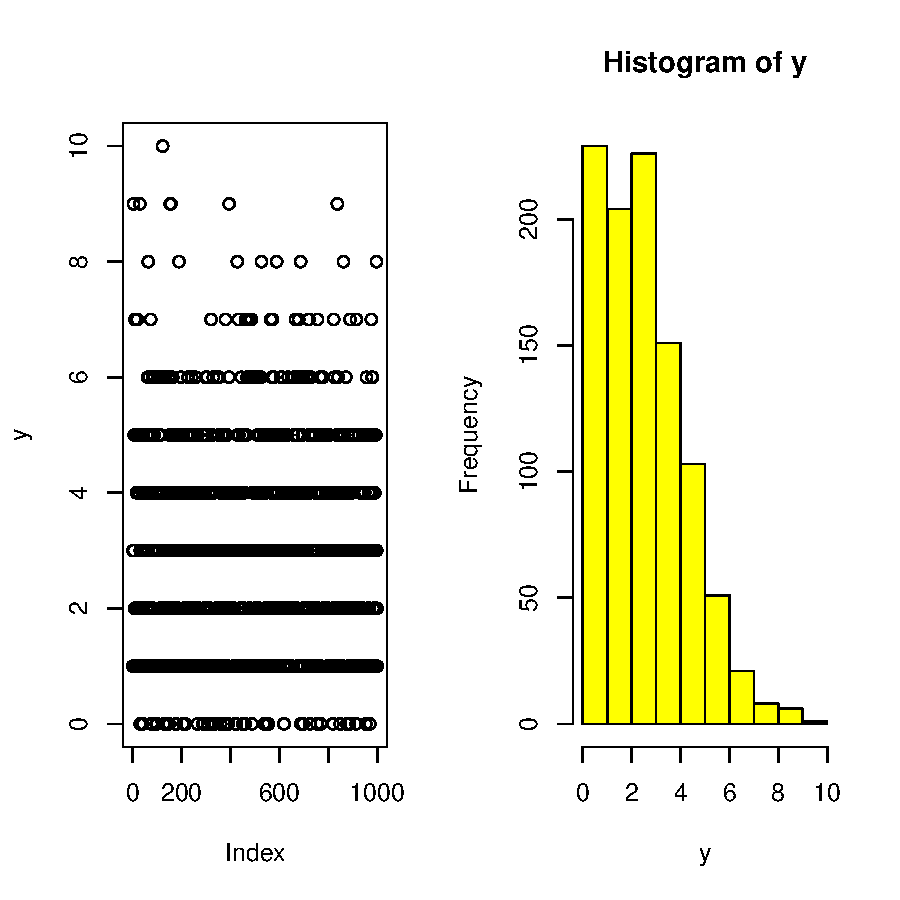
\includegraphics{HW1-007}
\end{figure}

\clearpage
\item The square root transformation gives

\begin{figure}[H]
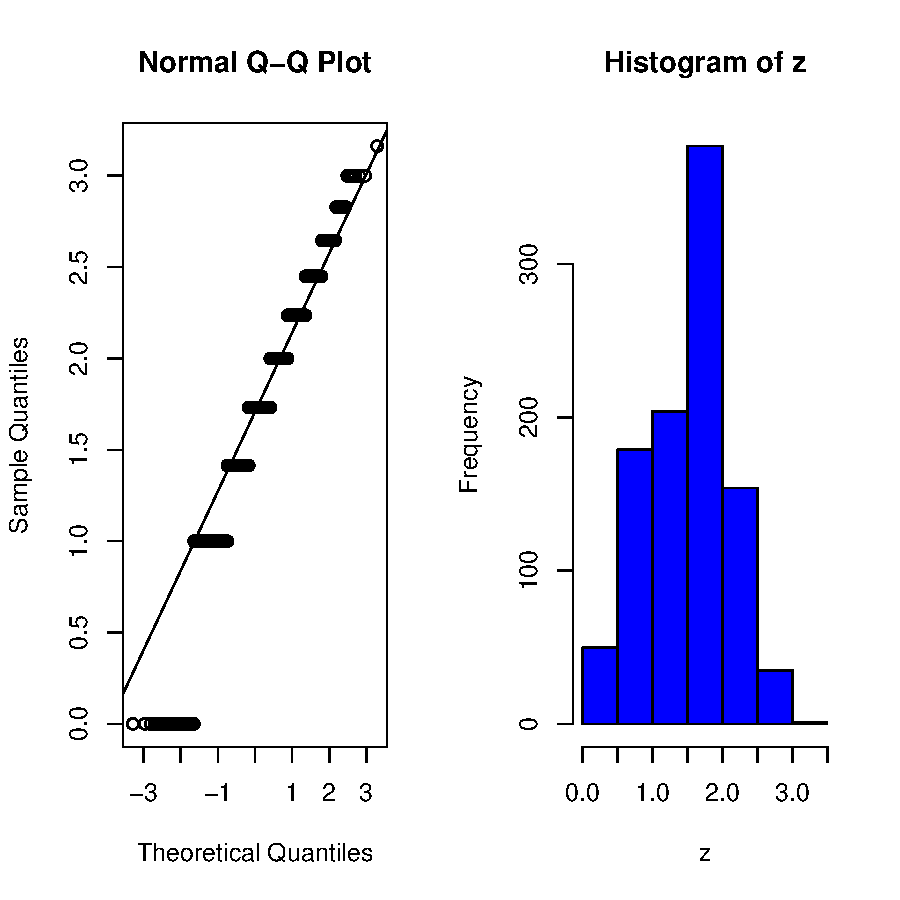
\includegraphics{HW1-008}
\end{figure}
\en
which seems very close to normal distribution.

% break
\clearpage
\section*{Answer 4}
\bn
\item Y$\sim$ Laplace$(\mu, \sigma), y\in R$\\
Pdf of Y is\\
$f(y)=\frac{1}{2\sigma}e^{-\frac{|(y-\mu)|}{\sigma}}, y\in R$\\
Now the mean can be evaluated as 
\begin{equation*}
\begin{aligned}
E[Y] &= \int_{-\infty}^{+\infty} \!yf(y)\ \mathrm{d}y \\
&= \int_{-\infty}^{+\infty} \!y\frac{1}{2\sigma}e^{-\frac{|(y-\mu)|}{\sigma}}\ \mathrm{d}y \\
&= \frac{1}{2\sigma}\left[\int_{-\infty}^{\mu}\!ye^{\frac{y-\mu}{\sigma}}\ \mathrm{d}y+\int_{\mu}^{+\infty}\!ye^{-\frac{y-\mu}{\sigma}}\ \mathrm{d}y\right]\\
&= \frac{1}{2\sigma}\left\{\left[y \sigma e^{\frac{y-\mu}{\sigma}} |_{-\infty}^{\mu}-\int_{-\infty}^{\mu}\!\sigma e^{\frac{y-\mu}{\sigma}}\ \mathrm{d}y\right]+\left[y (-\sigma) e^{-\frac{y-\mu}{\sigma}} |_{\mu}^{+\infty}-\int_{\mu}^{+\infty}\!(-\sigma) e^{-\frac{y-\mu}{\sigma}}\ \mathrm{d}y\right]\right\}\\
&= \frac{1}{2}\left\{\left[\mu-\sigma e^{\frac{y-\mu}{\sigma}}|_{-\infty}^{\mu}\right]+\left[\mu+(-\sigma) e^{-\frac{y-\mu}{\sigma}}|_{\mu}^{+\infty}\right]\right\}\\
&= \frac{1}{2}[(\mu-\sigma)+(\mu+\sigma)]\\
&= \mu
\end{aligned}
\end{equation*}
Similarily $E[X^2]$ can be evaluated and it comes out to be $\mu^2+2\sigma^2$. Thus
\begin{equation*}
\begin{aligned}
Var[Y]&=\mu^2+2\sigma^2-\mu^2\\
&= 2\sigma^2
\end{aligned}
\end{equation*}

\item The set of parameters $(\mu, \sigma)$ that make $E[Y]=3$ and $Var[Y]=1$ are $(3,\frac{1}{\sqrt{2}})$.

\item If $E[Y]=\mu=3, Var[Y]=2\sigma^2=1$, the plots of the simulated random variables and the histogram are given as:

\begin{figure}[H]
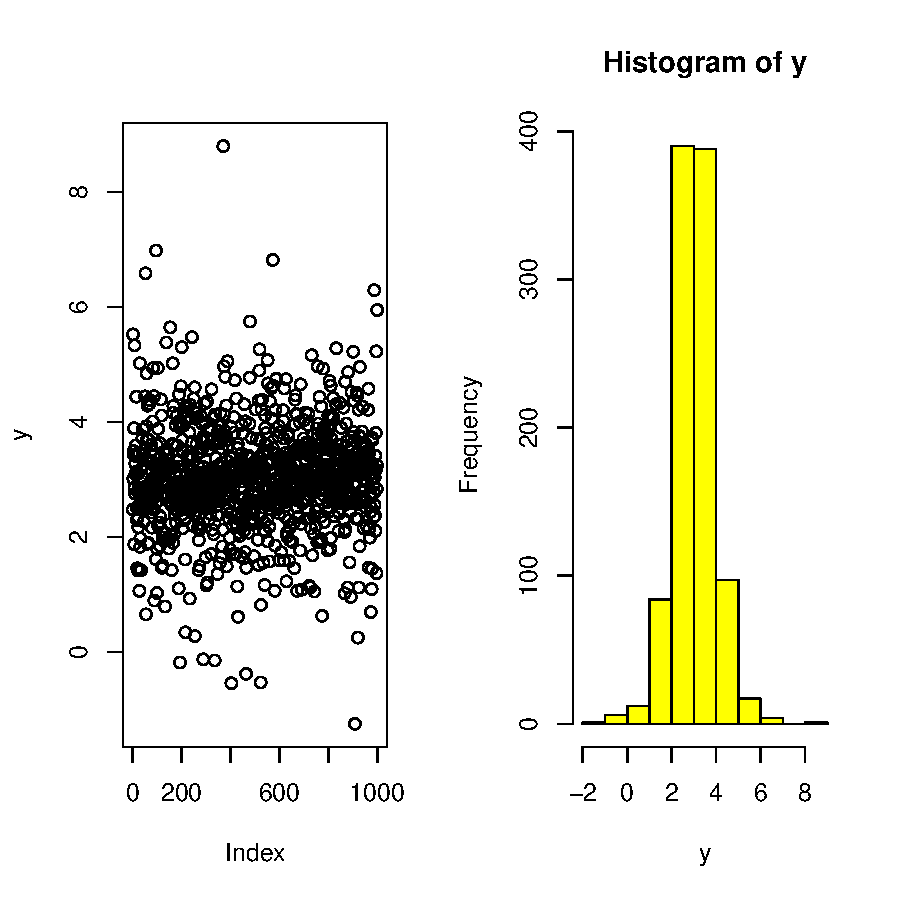
\includegraphics{HW1-009}
\end{figure}

\clearpage
\item The square root power transformation gives the following plots:
\begin{figure}[H]
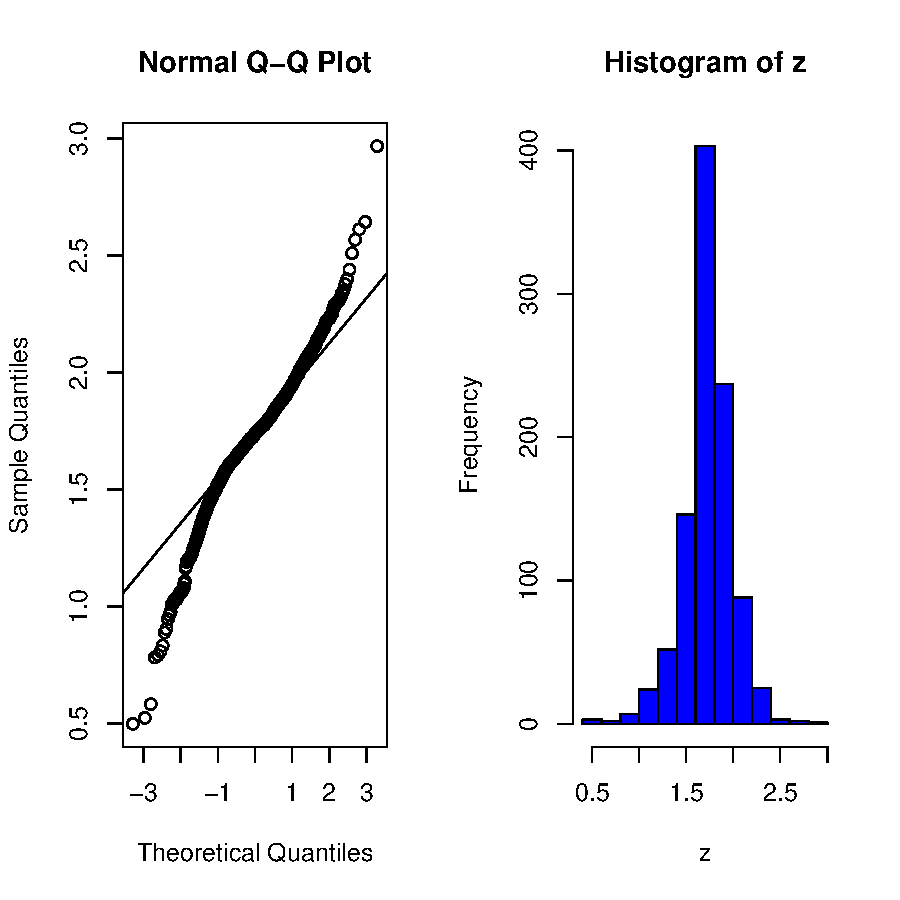
\includegraphics{HW1-010}
\end{figure}

\clearpage
The cube root power transformation gives the following plots:
\begin{figure}[H]
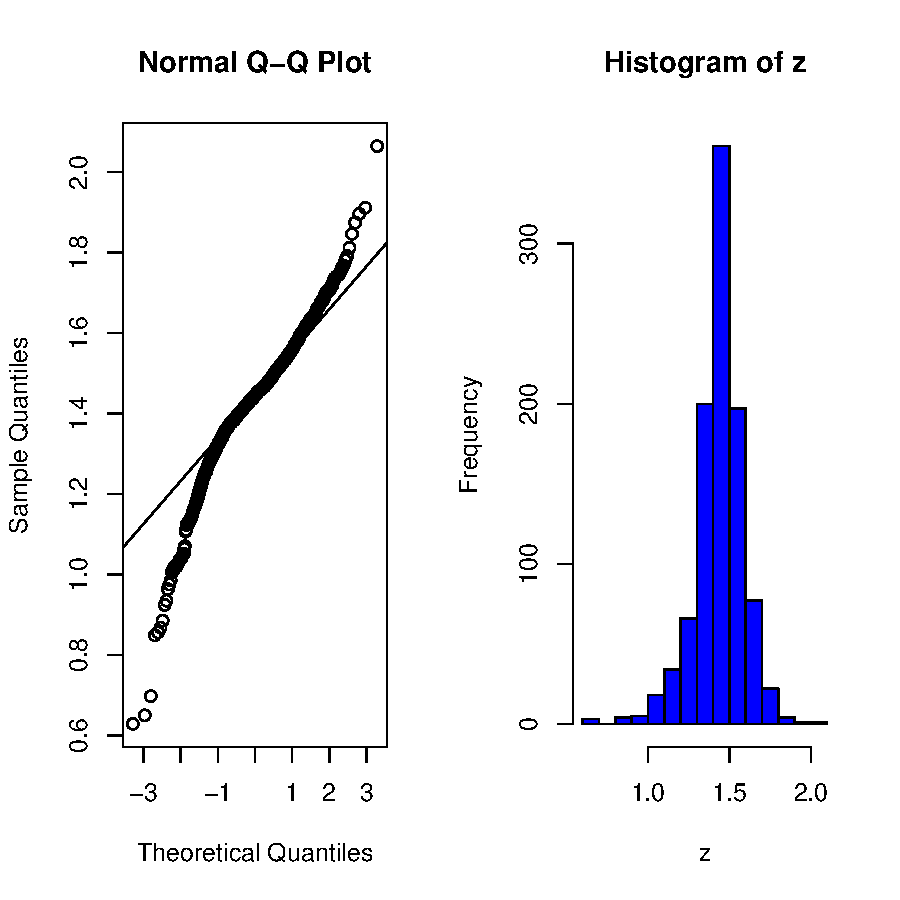
\includegraphics{HW1-011}
\end{figure}
\en

%break
\clearpage
\section*{Answer 5}
\bn
\item 
Plotting the histogram for the interarrival data:

\begin{figure}[H]
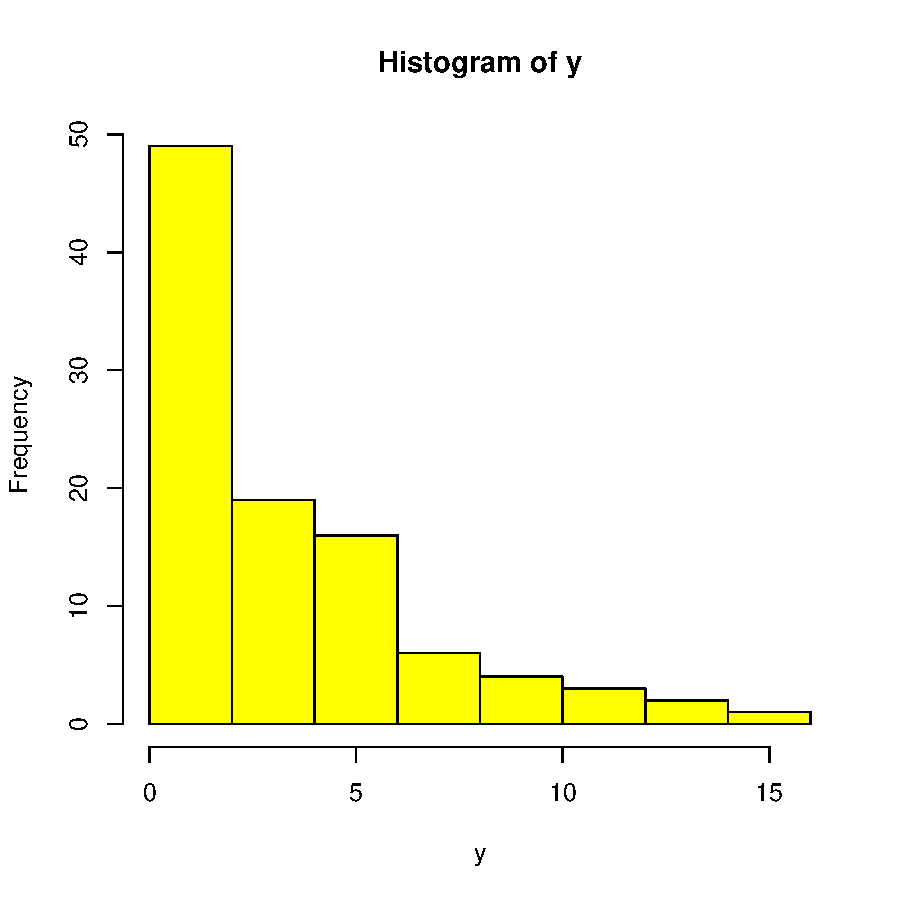
\includegraphics{HW1-012}
\end{figure}

From the histogram, it is clear that the support is $R^{+}$. The shape of the ditribution indicates that it is exponential. Now the exponential distribution has one parameter $\mu$ with the pdf as:\\
$f(x)=\frac{1}{\mu}e^{-\frac{x}{\mu}}$\\
The theoretical mean and variance are given as:\\
$E[X]=\mu$ and $Var[X]=\mu^2$
The sample mean and variance are
\begin{Schunk}
\begin{Soutput}
[1] 3.285651
\end{Soutput}
\begin{Soutput}
[1] 11.05406
\end{Soutput}
\end{Schunk}
respectively.\\
Comparing the sample mean and the theoretical mean, we get the parameter value $\mu=3.285651$\\

\item 
The data clearly shows that all the sample values are greater than zero. They lie in the following range:
\begin{Schunk}
\begin{Soutput}
[1] 0.0405379
\end{Soutput}
\begin{Soutput}
[1] 15.35806
\end{Soutput}
\end{Schunk}
i.e. the sample data has the support as [0.0405379,15.35806]. This is a subset of the theoretical support $R^{+}\cup \left\{0\right\} $.\\
Further, the theoretical mean $\mu$ is taken to be equal to the sample mean under the proposed model. The theoretical variance $\mu^2$ is again taken equal to the sample variance under the proposed model.
\item
Now $P(X>x)=e^{-\frac{x}{\hat{\mu}}}$. Thus $P(X>15)$ comes out to be 
\begin{Schunk}
\begin{Soutput}
[1] 0.0104067
\end{Soutput}
\end{Schunk}
\en

%break
\clearpage
\section*{Answer 6}
\bn
\item 
Plotting the histogram for the cars data:

\begin{figure}[H]
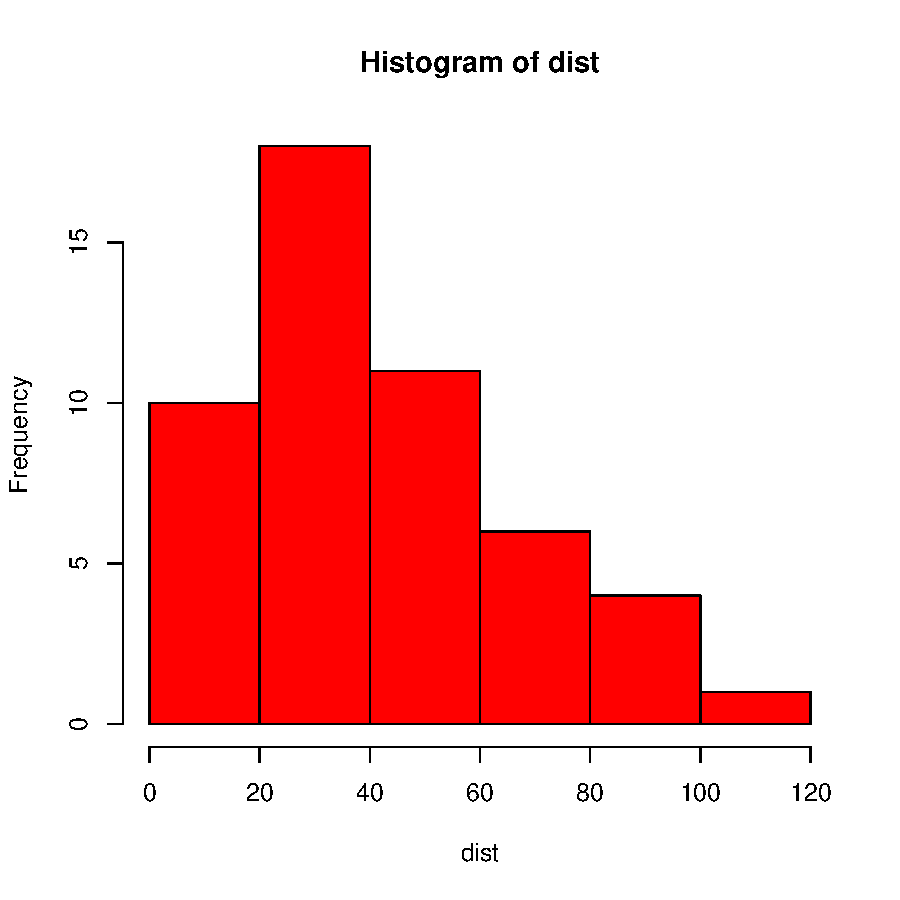
\includegraphics{HW1-016}
\end{figure}

From the histogram, it is clear that the support is $R^{+}$. The shape of the ditribution indicates that gamma distribution would be appropriate.. Now the gamma distribution has two parameters $\alpha$ and $\beta$ with the pdf as:\\
$f(x)=\frac{\beta^{\alpha}}{\Gamma \alpha}e^{-\beta x}x^{(\alpha-1)}, x>0$\\
The theoretical mean and variance are given as:\\
$E[X]=\frac{\alpha}{\beta}$ and $Var[X]=\frac{\alpha}{\beta^2}$
The sample mean and variance are
\begin{Schunk}
\begin{Soutput}
[1] 42.98
\end{Soutput}
\begin{Soutput}
[1] 664.0608
\end{Soutput}
\end{Schunk}
respectively.\\
Comparing the sample mean and variance with the theoretical mean and variance, we get the parameter values as
\begin{Schunk}
\begin{Soutput}
[1] 2.781794
\end{Soutput}
\begin{Soutput}
[1] 0.06472299
\end{Soutput}
\end{Schunk}

\item 
The data clearly shows that all the sample values are greater than zero. They lie in the following range:
\begin{Schunk}
\begin{Soutput}
[1] 2
\end{Soutput}
\begin{Soutput}
[1] 120
\end{Soutput}
\end{Schunk}
i.e. the sample data has the support as [2,120]. This is a subset of the theoretical support $R^{+}$.\\
Further, the theoretical mean is taken to be equal to the sample mean under the proposed model. The theoretical variance is again taken equal to the sample variance under the proposed model.
\item
$P(X>80)$ comes out to be 
\begin{Schunk}
\begin{Soutput}
[1] 0.08919011
\end{Soutput}
\end{Schunk}
The observed frequency is
\begin{Schunk}
\begin{Soutput}
[1] 0.1
\end{Soutput}
\end{Schunk}

\en

\section*{Answer 7}
\bn
\item
\begin{Schunk}
\begin{Soutput}
     [,1]
[1,]    5
[2,]    2
[3,]    0
[4,]   16
\end{Soutput}
\end{Schunk}
\item
\begin{Schunk}
\begin{Soutput}
     [,1]
[1,]    6
\end{Soutput}
\end{Schunk}
\item
\begin{Schunk}
\begin{Soutput}
     [,1] [,2] [,3]
[1,]    4    2   -2
[2,]    2    1   -1
[3,]   -2   -1    1
\end{Soutput}
\end{Schunk}
\item
\begin{Schunk}
\begin{Soutput}
     [,1] [,2] [,3]
[1,]   92   -9   20
[2,]   -9   31    8
[3,]   20    8   18
\end{Soutput}
\end{Schunk}
\item
\begin{Schunk}
\begin{Soutput}
[1] 141
\end{Soutput}
\end{Schunk}
\item
\begin{Schunk}
\begin{Soutput}
            [,1]        [,2]        [,3]
[1,]  0.01720655  0.01121560 -0.02410310
[2,]  0.01121560  0.04374782 -0.03190526
[3,] -0.02410310 -0.03190526  0.09651689
\end{Soutput}
\end{Schunk}
\en
\end{document}
